\ifx\wholebook\relax \else

\documentclass[b5paper]{article}
\usepackage[nomarginpar
  %, margin=.5in
]{geometry}

\addtolength{\oddsidemargin}{-0.05in}
\addtolength{\evensidemargin}{-0.05in}
\addtolength{\textwidth}{0.1in}

\usepackage[en]{../prelude}

\setcounter{page}{1}

\begin{document}

\title{Numbers}

\author{Xinyu LIU
\thanks{{\bfseries Xinyu LIU} \newline
  Email: liuxinyu95@gmail.com \newline}
  }

\maketitle
\fi

\markboth{Numbers}{Mathematics of Programming}

\ifx\wholebook\relax
\chapter{Numbers}
\numberwithin{Exercise}{chapter}
\fi

\epigraph{Numbers are the highest degree of knowledge. It is knowledge itself.}{--Plato}

\section{The history of number}

%\begin{wrapfigure}{R}{0.3\textwidth}
\begin{figure}[htbp]
 \centering
 \includegraphics[scale=0.36]{img/clay-envelope}
 \caption{The envelop of tokens in Uruk period from Susa. Louvre Museum}
 \label{fig:clay-token}
\end{figure}
%\end{wrapfigure}

The number emerged with human evolution. Some people believe that language was inspired by numbers. Our ancestors learned the numbers from the gathering and hunting activities. People needed to count the gathered fruits. As trading developed, people needed numeral tools to handle bigger numbers than previously encountered.

We found in the regions of Iran, people made clay tokens for record keeping around 4000 BC. they created two round tokens with `+' sign baked to represent "two sheep". Each token represented a sheep. Representing a hundred sheep with many tokens would be impractical, so they invented different clay tokens to represent ten sheep, twenty sheep and so on. In order to avoid the record being altered, people invented a clay envelope in which tokens were placed, sealed, and baked. If anybody disputed the number, they could break open the envelope and do a recount. They also pressed the signs outside the envelop before it was baked, these signs on the outside became the first written language for numbers\cite{Calvin-Clawson-1994}. \Cref{fig:clay-token} shows the ancient clay tokens and envelopes found in Uruk period.

As the number increasing, the clay tokens and envelops were gradually replaced by more powerful numerals. About 3500 BC, the Sumerians in Mesopotamia used round stylus in flat clay tablets to carve pictographs representing various tokens. Each sign represented both commodity being counted and the quantity of that commodity.

The next big step happened around 3100 BC. The abstract numbers dissociated from the thing being counted. We found from the clay tablets, the things being counted were indicated by pictographs carved with a sharp stylus next to round-stylus numerals. These abstracted numerals later evolved to Babylonian cuneiform characters.

%\begin{wrapfigure}{R}{0.5\textwidth}
\begin{figure}[htbp]
 \centering
 \subcaptionbox{Babylonian numerals\cite{wiki-babylonian-num}}[0.45\linewidth]{
   \includegraphics[scale=0.36]{img/Babylonian_numerals}} \quad \quad
 \subcaptionbox{The abstract three}[0.45\linewidth]{
   \includegraphics[scale=0.21]{img/abstract-num}}
 \captionsetup{labelformat=empty}
 \label{fig:babylonian-num}
 \label{fig:abstract-num}
\end{figure}
%\end{wrapfigure}

The abstract number emerged from intelligent mind. People realized the abstract three could represent three eggs, three trees, and three jars. It's a powerful tool. People can manipulate the pure numbers and apply the result to the concrete things. When increase the abstract three by one to get four, we know gathering another egg after three egges gives four eggs; we also know baking another jar after three jars gives four jars. We resolve a whole kind of problems instead of one by one.

Starting from the numbers, people developed add, subtraction, then the more powerful methods of multiplication and division. When measure the length, angles, areas, and volumes, we connected the number to the geometry quantity. People from different places found the inner relationships and laws for the numbers and shapes. Ancient Egyptian, Greece, and Chinese people found the Pythagoras theorem independently, and applied it to the amazing works like to build the great pyramid. Trace back from the modern civilization, we find the natural number is the source of math and science. German mathematician Kronecker said `God made the integers; all else is the work of man.'\footnote{Natural number is different from integer. We'll come back to the story of Kronecker in the chapter of infinity.}


\section{Peano Axioms}

Euclid's {\em Element} is the first work introduced the axiomatic methods. From five axioms and postulates, Euclid developed the laws one by one elaborately. Every result is only based on the axioms and the theorems proved before. With this approach, he built the great building of geometry. However, there was no axiomatic formal system for natural numbers for long time. People considered natural numbers were straightforward and the related facts were obvious. The axioms of natural number was setup by Italian mathematician Peano till 1889. known as Peano Axioms nowadays. It's interesting that there are also five axioms.

\begin{enumerate}
\item 0 is a natural number. Expressed as $0 \in N$;
\item For every natural number, there is a successor natural number. Expressed as $n' = succ(n)$;
\end{enumerate}

It seems that we can define the infinite natural numbers only with these two axioms. From 0, the next is 1, then 2, 3, ..., $n$, and $n+1$, ... However, there is a counter example. Consider a set with only two numbers $\{0, 1\}$. Where the successor of 1 is defined as 0, while the successor of 0 is defined as 1. It satisfies the above two axioms well although they are not as we expected. In order to avoid this situation, we need the third Peano axiom.

\begin{enumerate}
  \setcounter{enumi}{2}
  \item 0 isn't the successor of any natural number. Expressed as $\forall n \in N: n' \neq 0$;
\end{enumerate}

Are these three axioms enough? We can still find another counter example. Consider the set of $\{0, 1, 2\}$. Define the successor of 0 is 1, the successor of 1 is 2, and the successor of 2 is 2 again. It satisfies all the three axioms so far. We therefore need the fourth Peano axiom.

\begin{enumerate}
  \setcounter{enumi}{3}
  \item Different natural numbers have different successors. In other words, if two natural numbers have the same successor, then they are same. Expressed as $n, m \in N$ if $n' = m'$ then $n = m$;
\end{enumerate}

However, it is still not enough. We can still find another example. For set \{0, 0.5, 1, 1.5, 2, 2.5, ...\}. Define 1 is the successor of 0, 2 is the successor of 1, ...; 1.5 is the successor of 0.5, 2.5 is the successor of 1.5, ...; But 0.5 is not the successor of any other numbers. In order to exclude such `unreachable' elements, we need the last Peano axiom.

\begin{enumerate}
  \setcounter{enumi}{4}
  \item If some subset of natural numbers contains 0, and every element in it has a successor, then this subset is same as the whole natural numbers. Expressed as if $S \subset N: 0 \in S$ and $\forall n \in S$ if $n' \in S$ then $S = N$.
\end{enumerate}

Why does the fifth axiom exclude the above counter example? For \{0, 0.5, 1, 1.5, 2, 2.5, ...\}, consider the subset of \{0, 1, 2, ...\}. 0 belongs to it, and every element has a successor. But it is not identical to the original set. As 1.5, 2.5, ... are not in this subset, it does not satisfy the fifth Peano axiom. This last axiom as also known as `Axiom of induction'. It can be equally stated as the following.

\begin{enumerate}
  \setcounter{enumi}{4}
  \item For any proposition of natural numbers, if it holds for 0, and when assume it holds for some number $n$, we can prove it also holds for $n'$, then the proposition holds for all natural numbers. (This axiom ensure the correctness of mathematical induction.)
\end{enumerate}

This the complete statement of the five Peano axioms. They can build the first-order arithmetic, also known as Peano arithmetic\footnote{Some people use 1, but not 0 as the first natural number. The order is different from the original works published by Peano, where the fifth axiom of induction was list as the third one.}.

%\begin{wrapfigure}{R}{0.4\textwidth}
\begin{figure}[htbp]
 \centering
 \includegraphics[scale=0.2]{img/Peano}
 \caption{Giuseppe Peano (1858-1932)}
 \label{fig:Peano}
\end{figure}
%\end{wrapfigure}

Giuseppe Peano was an Italian mathematician, logician, and linguist. Peano was born and raised on a farm at Spinetta, a hamlet now belonging to Cuneo, Italy. He enrolled at the University of Turin in 1876, graduating in 1880 with high honors, after which the University employed him to teach calculus course. In 1887, Peano married Carola Crosio. In 1886, he began teaching concurrently at the Royal Military Academy. From 1880s, Peano started to study mathematical logic. He published the Peano axioms, a formal foundation for the natural numbers. Peano started the Formulario Project. It was to be an ``Encyclopedia of Mathematics'', containing all known formulae and theorems of mathematical science. In 1900, the Second International Congress of Mathematicians was held in Paris. At the conference Peano met Bertrand Russell and gave him a copy of Formulario. Russell was so struck by Peano's innovative logical symbols that he left the conference and returned home to study Peano's text\cite{M-Kline-2007}.

When Russell and Whitehead wrote {\em Principia Mathematica}, they were deeply influenced by Peano. Peano played a key role in the axiomatization of mathematics and was a leading pioneer in the development of mathematical logic and set theory. As part of this effort, he made key contributions to the modern rigorous and systematic treatment of the method of mathematical induction. He spent most of his career teaching mathematics at the University of Turin. He also wrote an international auxiliary language, Latino sine flexione ("Latin without inflections", later called Interlingua), which is a simplified version of Classical Latin. Most of his books and papers are in Latino sine flexione. Although Peano put a lot of effort to rewrite his works in the new language, few people read it. On the other hand, his early works in French influnced many mathematicians, especially to the Bourbaki group, which came out many top mathematicians like André Weil, Jean Dieudonné, Henri Cartan, Schwartz, Serre, Grothendieck and so on. Giuseppe Peano died on April, 20th, 1932 when he suffered a fatal heart attack.

\section{Natural numbers and programming}

People make amazing achievement with the modern computer systems. We didn't establish the axioms of computer programming before developing these results. After the great success of computer application, then the foundation of computer science is gradually developed to be strict, formal, and mathematized. The similar thing happens several times in our history. Calculus was developed by Newton and Leibniz independently in the 17th century, then applied to a wide range of areas, including fluid dynamics, astronomy and so on. However, it was not formalized until Weierstrass and Cauchy developed the foundation in the 19th century\cite{M-Kline-2007}.

We'll emulate it. From the Peano axioms, define the natural numbers with computer programs. In a computer system without familiar numbers like 0, 1, 2, ..., we can define the natural numbers as below\footnote{We use a virtual, ideal programming language in this book. Some real programs are given at the end of each chapter for reference.}:

\begin{Haskell}
data Nat = zero | succ Nat
\end{Haskell}

%% \[
%% N \triangleq zero | succ(N)
%% \]

A natural number is either zero, or the successor of another natural number. Symbol `|' is mutual exclusive, it implicates the axiom that zero is not the successor of any natural number. We can further define the addition for natural numbers.

\begin{Haskell}
a + zero = a
a + (succ b) = succ (a + b)
\end{Haskell}

There are two rules for addition. First, any natural number adds zero gives that number itself; second, a natural number adds to a successor of some natural number equals to the successor of the sum of the two. In mathematic expression:

\be
\begin{array}{l}
a + 0 = a \\
a + b' = (a + b)'
\end{array}
\ee

Let's use 2+3 as the example. natural number 2 is succ(succ zero), and 3 is succ(succ(succ zero)). According to the definition of addition:

\begin{Haskell}
  succ(succ zero) + succ(succ(succ zero))
= succ(succ(succ zero) + succ(succ zero))
= succ(succ(succ(succ zero) + succ zero))
= succ(succ(succ(succ(succ zero) + zero)))
= succ(succ(succ(succ(succ zero))))
\end{Haskell}

The result is the 5th successor of zero. It's not practical to apply succeed function again and again for big numbers like 100. Let's introduce a simplified notation for natural number $n$.

\be
n = foldn(zero, succ, n)
\ee

It applies $succ$ function to zero $n$ times. Function $foldn$ can be realized as the following.

\be
\begin{array}{l}
foldn(z, f, 0) = z \\
foldn(z, f, n') = f(foldn(z, f, n))
\end{array}
\label{eq:foldn}
\ee

Function $foldn$ defines some operation on natural number. When $z$ is $zero$, and $f$ is the $succ$ function, then it can apply the succeed operation multiple times to get a specific natural number. We can verify it with the first several numbers.

\begin{Haskell}
foldn(zero, succ, 0) = zero
foldn(zero, succ, 1) = succ(foldn(zero, succ, 0)) = succ zero
foldn(zero, succ, 2) = succ(foldn(zero, succ, 1)) = succ(succ zero)
...
\end{Haskell}

Multiplication for natural number can be defined on top of addition.

\begin{Haskell}
a *'.'* zero = zero
a *'.'* (succ b) = a *'.'* b + a
\end{Haskell}

The multiplication can be expressed in mathematic symbols as below.

\be
\begin{array}{l}
a \cdot 0 = 0 \\
a \cdot b' = a \cdot b + a
\end{array}
\ee

%\begin{wrapfigure}{R}{0.4\textwidth}
\begin{figure}[htbp]
\centering
\begin{tikzpicture}[scale=0.8]
\filldraw[fill=gray, draw=black, pattern=north west lines] (0, 0) rectangle (2, 1)
    (2, 0) rectangle (3, 1);
\draw (3, 0) rectangle (4.5, 1);
\draw (0, -1) rectangle (2, -2);
\filldraw[fill=gray, draw=black, pattern=north west lines] (2, -1) rectangle (3, -2)
    (3, -1) rectangle (4.5, -2);
\end{tikzpicture}
\caption{Association of addition in geometry. The areas of the above and bottom are same.}
%\end{wrapfigure}
\end{figure}

It turns out that the associative and commutative laws for addition and multiplication are neither axioms nor postulations. They all can be proved by Peano axioms and the definitions. Let's prove the associative law for addition as an example. This law states $(a + b) + c= a + (b + c)$. We firstly prove it holds when $c=0$. According to the first rule in the add definition:

\[
\begin{array}{rl}
(a + b) + 0 & = a + b \\
            & = a + (b + 0)
\end{array}
\]

Then for induction, assume $(a + b) + c = a + (b + c)$ hold, we want to prove $(a + b) + c' = a + (b + c')$.

\[
\begin{array}{rlr}
(a + b) + c' & = (a + b + c)' & \text{2nd equation defining +, (backward)} \\
             & = (a + (b + c))' & \text{induction assumption} \\
             & = a + (b + c)' & \text{2nd equation defining +} \\
             & = a + (b + c') & \text{2nd equation defining +, (backward)}
\end{array}
\]

Hence proves the associative law for addition. However, it is a bit complex to prove the commutative law. We give it in the Appendix of the book.

%\begin{wrapfigure}{R}{0.4\textwidth}
\begin{figure}[htbp]
\centering
\begin{tikzpicture}[scale=0.8]
\draw (0, 0) rectangle (2, 1)
    (2, 0) rectangle (3, 1);
\draw (0, -1) rectangle (1, -2)
    (1, -1) rectangle (3, -2);
\end{tikzpicture}
\caption{Commutative law of addition in geometry. Turn upside down or mirror the upper figure.}
\end{figure}
%\end{wrapfigure}

\begin{Exercise}\label{ex:Peano-axiom}
\Question{Define 1 as the successor of 0, prove $a \cdot 1 = a$ holds for all natural numbers;}
\Question{Prove the distributive law for multiplication;}
\Question{Prove the associative and commutative laws for multiplication.}
\Question{How to verify 3 + 147 = 150 with Peano axioms?}
\Question{Give the geometric explanation for distributive, associative, and commutative laws of multiplication.}
\end{Exercise}

\begin{Answer}[ref={ex:Peano-axiom}]
\Question{Define 1 as the successor of 0, prove $a \cdot 1 = a$ holds for all natural numbers;

We first use mathematical induction to prove $0 + a = a$ (refer to {\em Appendix - Proof of commutative law of addition}). Then:

\[
\begin{array}{rlr}
a' \cdot 1 & = a' \cdot 0' & \text{1 as the successor of 0} \\
           & = a' \cdot 0 + a' & \text{2nd rule of multiplication} \\
           & = 0 + a' & \text{1st rule of multiplication} \\
           & = a' & \text{proved previously}
\end{array}
\]
}

\Question{Prove the distributive law for multiplication;

\begin{proof}
We can prove the left side distribution law $c(a + b) = ca + cb$ by mathematical induction. First when $b = 0$:

\bre
c(a + 0) & = & ca & \text{1st rule of addition} \\
         & = & ca + 0 & \text{reverse of 1st rule of addition} \\
         & = & ca + c0 & \text{reverse of 1st rule of multiplication} \\
\ere

Next suppose $c(a + b) = ca + cb$ holds, we need prove $c(a + b') = ca + cb'$

\bre
c(a + b') & = & c(a + b)' & \text{2nd rule of addition} \\
          & = & c(a + b) + c & \text{2nd rule of multiplication} \\
          & = & ca + cb + c & \text{induction hypothesis} \\
          & = & ca + (cb + c) & \text{associative law of addition} \\
          & = & ca + cb' & \text{reverse of 2nd rule of multiplication} \\
\ere
\end{proof}
}

\Question{Prove the associative and commutative laws for multiplication.

We only prove the associative law for multiplication $(ab)c = a(bc)$. For the commutative law, we provide a proof outline.

Using mathematical induction, when $c = 0$:

\bre
(ab)0 & = & 0 & \text{1st rule of multiplication} \\
      & = & a0 & \text{reverse of 1st rule of multiplication} \\
      & = & a(b0) & \text{reverse of 1st rule of multiplication} \\
\ere

Next suppose $(ab)c = a(bc)$, we need prove $(ab)c' = a(bc')$

\bre
(ab)c' & = & (ab)c + ab & \text{2nd rule of multiplication} \\
       & = & a(bc) + ab & \text{induction hypothesis} \\
       & = & a(bc + b) & \text{distribution law proven above} \\
       & = & a(bc') & \text{reverse of 2nd rule of multiplication} \\
\ere

To prove the commutative law of multiplication, we take three steps, all with mathematical induction. First we prove $1a = a$, then prove the right side distribution law $(a + b)c = ac + bc$, finally, prove the commutative law.
}

\Question{How to verify 3 + 147 = 150 with Peano axioms?

Let us first see the classic proof of 2 + 2 = 4:

\bre
2 + 2 & = & 0'' + 0'' & \text{2 is the successor of successor of 0} \\
      & = & (0'' + 0')' & \text{2nd rule of addition} \\
      & = & ((0'' + 0)')' & \text{2nd rule of addition} \\
      & = & ((0'')')' & \text{1st rule of addition} \\
      & = & 0'''' = 4 & \text{4 times successor of 0} \\
\ere

It will be too long to prove 3 + 147 = 150 in this way. One method is to apply the commutative law of addition, then prove 147 + 3 = 150; another method is to use the mathematical induction to prove $3 + a = a'''$
}

\Question{Give the geometric explanation for distributive, associative, and commutative laws of multiplication.

See \cref{fig:geometric-arithmetic}

%\begin{figure}[htbp]
\begin{center}
 \includegraphics[scale=0.35]{../appendix/answer/img/geometric-arithmetic}
  % \captionsetup{labelformat=empty}
 \captionof{figure}{Geometric explanation for arithmetic laws}
 \label{fig:geometric-arithmetic}
\end{center}
%\end{figure}
}
\end{Answer}

\section{Structure of natural numbers}

We can define more complex operations on top of addition and multiplication. One example is summation: $0 + 1 + 2 + ... $

\be
\begin{array}{l}
sum(0) = 0 \\
sum(n + 1) = (n + 1) + sum(n)
\end{array}
\ee

Another example is the factorial $n!$

\be
\begin{array}{l}
\textit{fact}(0) = 1 \\
\textit{fact}(n + 1) = (n + 1) \cdot \textit{fact}(n)
\end{array}
\ee

They are similar to each other. Although artificial intelligence achieves incredible result today, the machine can't jump out of the system, as intelligent mind, to abstract in a higher level. This is one of the most complex, powerful, and mysterious part in human brain\cite{GEB}.

Corresponding to zero in natural number, both summation and factorial have a start value. Summation starts from zero, factorial starts from one. For recursion, they both apply some operation to a number and its successor. For summation, it's $n' + sum(n)$, for factorial, it's $n' \cdot \textit{fact}(n)$. If we abstract the start value as $c$, the recursive operation as $h$, then we can use the same form for both.

\be
\begin{array}{l}
f(0) = c \\
f(n + 1) = h(f(n))
\end{array}
\ee

This scheme is called as {\em structural} recursion over the natural numbers. Below examples show how it behaves over the first several numbers.

\vspace{5mm}

\begin{tabular}{l|l}
$n$ & $f(n)$ \\
\hline
0 & $c$ \\
1 & $f(1) = h(f(0)) = h(c)$ \\
2 & $f(2) = h(f(1)) = h(h(c))$ \\
3 & $f(3) = h(f(2)) = h(h(h(c)))$ \\
... & ... \\
$n$ & $f(n) = h^n(c)$
\end{tabular}

\vspace{5mm}

Where $h^n(c)$ means applying operation $h$ over $c$ for $n$ times. It's an instance of the more general {\em primitive} recursion(\cite{Bird97}, p5). Further, we can find it is related to the $foldn$ defined in \cref{eq:foldn}.

\be
f = foldn(c, h)
\ee

There are three variables in the original $foldn$ definition, why are there only two appeared? We can actually write it as $f(n) = foldn(c, h, n)$. When we bind the first two variables to $foldn$, it turns to be a new function accepts one argument. We can consider it as $foldn(c, h)(n)$.

We call $foldn$ the {\em fold} operation on natural numbers. When $c$ is $zero$ and $h$ is $succ$, we get a sequence of natural numbers:

\[
zero, succ(zero), succ(succ(zero)), ... succ^n(zero), ...
\]

When $c$ and $h$ are other things than $zero$ or $succ$, then $foldn(c, h)$ describes some isomorphism\footnote{The formal definition of isomorphism will be given in later chapter. Different from the mathematic definition, here it means the similarity of the form.} to natural numbers. Here are some examples.

\[
(+ m) = foldn(m, succ)
\]

This is the operation to increase a number by $m$. When applying to the natural numbers, it generates an isomorphic sequence of $m, m + 1, m + 2, ..., n + m, ...$

\[
(\cdot m) = foldn(0, (+ m))
\]

This is the operation to multiply a number by $m$. When applying to the natural numbers, it generates an isomorphic sequence of $0, m, 2m, 3m, ..., nm, ...$

\[
m^{()} = foldn(1, (\cdot m))
\]

This is the operation to take the power for a number $m$. When applying to natural numbers, it generates an isomorphic sequence of $1, m, m^2, m^3, ..., m^n, ...$

Can we use the abstract tool $foldn$ to define the summation and factorial? Observe the below table.

\vspace{5mm}

\begin{tabular}{r|l|l|l|l|l|l}
$n$ & 0 & 1 & 2 & 3 & ... & $n'$ \\
\hline
$sum(n)$ & 0 & 1 + 0 = 1 & 2 + 1 = 3 & 3 + 3 = 6 & ... & $n' + sum(n)$ \\
\hline
$n!$ & 1 & 1 $\times$ 1 = 1 & 2 $\times$ 1 = 2 & 3 $\times$ 2 = 6 & ... & $n' \cdot (n!)$
\end{tabular}

\vspace{5mm}

We know that $h$ need to be a binary operation as it manipulates $n'$ and $f(n)$. To solve it, we define $c$ as a pair $(a, b)$\footnote{Also known as {\em tuple} in computer programs}. Then define some kind of `succ' operation on the pair. We also need functions to extract $a$ and $b$ from the pair.

\be
\begin{array}{l}
1st (a, b) = a \\
2nd (a, b) = b
\end{array}
\ee

With these setup, we can define summation:

\[
\begin{array}{ll}
c = (0, 0) & \text{Starting pair} \\
h (m, n) = (m', m' + n) & \text{Succeed the 1st; Add the successor and the 2nd} \\
sum = 2nd \circ foldn(c, h) \\
\end{array}
\]

Starting from $(0, 0)$, below table gives the steps for summation.

\vspace{5mm}

\begin{tabular}{r|l|l}
$(a, b)$ & $(a', b') = h (a, b)$ & $b'$\\
\hline
(0, 0) & (0 + 1 = 1, 1 + 0 = 1) = (1, 1) & 1 \\
(1, 1) & (1 + 1 = 2, 2 + 1 = 3) = (2, 3) & 3 \\
(2, 3) & (2 + 1 = 3, 3 + 3 = 6) = (3, 6) & 6 \\
... & ... & ... \\
$(m, sum(m))$ & $(m + 1, m + 1 + sum(m))$ & $sum(m + 1)$
\end{tabular}

\vspace{5mm}

Similarly, we can define factorial with $foldn$.

\[
\begin{array}{lr}
c = (0, 1) & \text{Starting pair for factorial} \\
h (m, n) = (m', m'n) & \text{Iteration for factorial} \\
fact = 2nd \circ foldn(c, h) \\
\end{array}
\]

Here we use the symbol `$\circ$' to `connect' the $2nd$ function and the $foldn(c, h)$ function. We call it {\em function composition}. $f\circ g$ means firstly apply $g$ to the variable, then apply $f$ on top of the result. That is $(f\circ g)(x) = f(g(x))$.

\index{Fibonacci}
\begin{figure}[htbp]
 \centering
 \includegraphics[scale=0.35]{img/Fibonacci}
 \caption{Leonardo Pisano, Fibonacci (1175-1250)}
 \label{fig:Fibonacci}
\end{figure}

Let's see another example powered by this abstract tool, Fibonacci sequence. It's named after the medieval mathematician Leonardo Pisano. Fibonacci originates from `filius Bonacci' in Latin. It means the son of (the) Bonacci. Fibonacci's father was a wealthy Italian merchant
 often did trading around North Africa and the Mediterranean coast. Fibonacci traveled with him as a young boy. It was in Bugia (now Béjaïa, Algeria) that he learned about the Hindu–Arabic numeral system. Fibonacci realized many advantage of this numeral system. He introduced it to Europe through his book, the {\em Liber Abaci} (Book of Abacus or Book of Calculation, 1202). European people were using Roman numeral system before that. We can still see Roman numbers in clock plat today. The Roman number for year 2018 is MMXVIII. Where M stands for 1000, so two M letters mean 2000; X represents 10, V stands for 5, the three I mean 3. Sum them up, we get 2018. The Hindu-Arabic numeral system introduced by Fibonacci is a positional decimal numeral system. We are using it almost everywhere today. It uses the zero invented by Indian mathematicians. Numbers at different position mean different value. This advanced numeral system were widely used in business, for example converting different currencies, calculating profit and interest, which were important to the growing banking industry. It influenced the mathematics in Europe greatly.

Fibonacci numbers is well known as a problem described in the {\em Liber Abaci}, although it can be traced back to 200 BC in India. Assuming a newly born pair of rabbits, one male, one female, are put in a field; rabbits are able to mate at the age of one month so that at the end of its second month a female can produce another pair of rabbits; rabbits never die and a mating pair always produces one new pair (one male, one female) every month from the second month on. Then how many pairs will there be in one year?

When start, there is a pair in the first month. In the second month, there is a new born pair. In total there are two pairs. In the third month, the matured pair produces another pair, while the new born in the previous month are still young. In total, there are 2 + 1 = 3 pairs. In the fourth month, the two pairs of matured rabbits produce another two pairs of baby. Plus the three pairs in the third month, there are total 3 + 2 = 5 pairs. Repeating it gives a sequence of numbers.

1, 1, 2, 3, 5, 8, 13, 21, 34, 55, 89, 144, ...

\begin{figure}[htbp]
 \centering
 \subcaptionbox{The length of the squares give a Fibonacci sequence}[0.45\linewidth]{
     \includegraphics[scale=0.35]{img/fibonacci_spiral}}
 \subcaptionbox{Dark: mature, Light: new born}[0.45\linewidth]{
     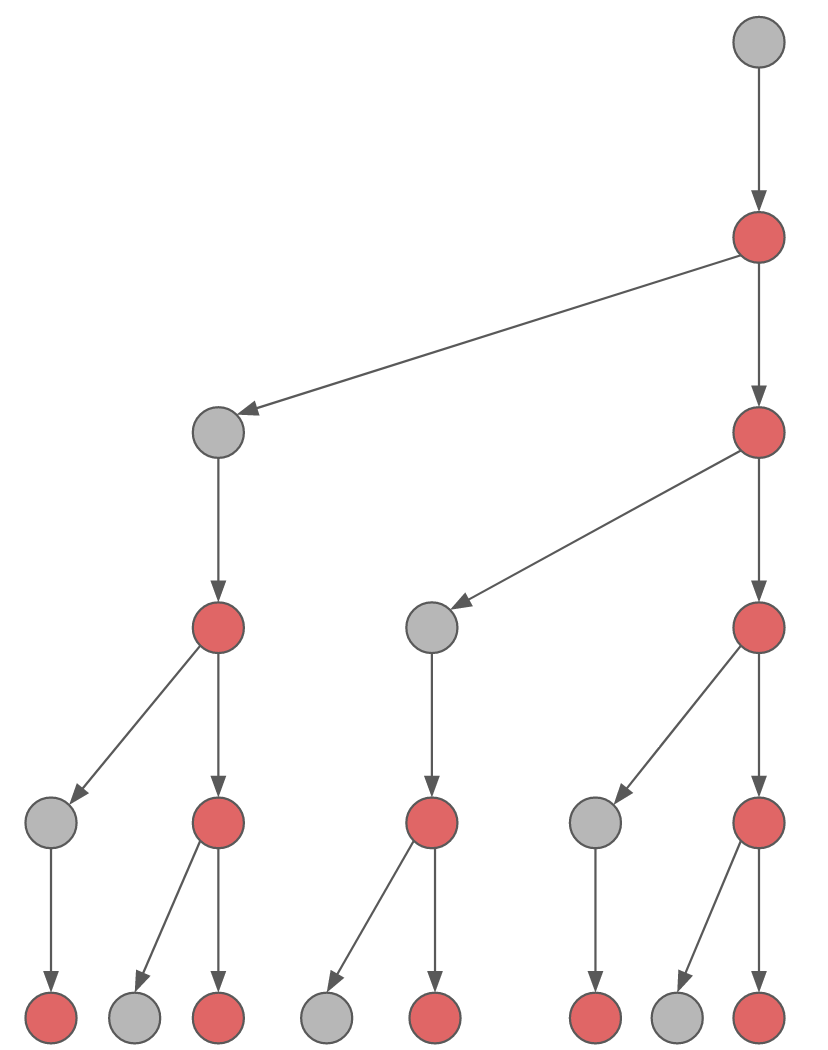
\includegraphics[scale=0.3]{img/Fibonacci-rabbits}}
 %\captionsetup{labelformat=empty}
 \caption{Expansion of Fibonacci numbers}
 \label{fig:fibonacci_spiral}
 \label{fig:Fibonacci-rabbits}
\end{figure}

It's easy to find the pattern of this sequence. From the third number, every number is the sum of the previous two. We can understand the reason behind it like this. Let there be $m$ pairs of rabbits in the previous month, and $n$ pairs in this month. As the new additional $n - m$ pairs are all new born, the rest $m$ pairs are mature. In the next month, the $n - m$ pairs grow mature; while the $m$ pairs of big rabbits produce another $m$ pairs of baby rabbits. The total pairs in the next month is the sum of big and baby rabbits, which is $(n - m) + m + m = n + m$. With this deduction, we can give the recursive definition of Fibonacci numbers.

\be
\begin{array}{l}
F_0 = 0 \\
F_1 = 1 \\
F_{n+2} = F_n + F_{n+1}
\end{array}
\ee

The starting numbers are defined as 0 and 1 by convention\footnote{If start from 1 and 3, it produces the Lucas sequence 1, 3, 4, 7, 11, 18, ...}. As Fibonacci numbers start from a {\em pair} of natural numbers, and the recursive relation also uses a pair of elements, we can use our abstract tool $foldn$ to define Fibonacci sequence\footnote{We'll give another different definition of Fibonacci numbers in the chapter about infinity.}.

\be
\begin{array}{l}
F = 1st \circ foldn((0, 1), h) \\
h (m, n) = (n, m + n)
\end{array}
\ee

Can this definition be realized in the computer programs in real world? Is it too idealistic? Below is a real piece of Haskell program implements Fibonacci numbers\footnote{After 2010, the n+k pattern matching is not supported any more in Haskell.}. Run command \texttt{fib 10} outputs the 10th Fibonacci number, 55\footnote{One line code to produce the first 100 Fibonacci numbers: \newline\texttt{take 100 \$ map fst \$ iterate ($\lambda$(m, n)->(n, m + n)) (0, 1)}}.

\begin{Haskell}[frame=single]
foldn z _ 0 = z
foldn z f n = f (foldn z f (n - 1))

fib = fst . foldn (0, 1) h where
  h (m, n) = (n, m + n)
\end{Haskell}

\begin{Exercise}\label{ex:foldn}
\Question{Define square for natural number $()^2$ with $foldn$;}
\Question{Define $()^m$ with $foldn$, which gives the $m$-power of a natural number;}
\Question{Define sum of odd numbers with $foldn$, what sequence does it produce?}
\Question{There is a line of holes (infinite many) in the forest. A fox hides in a hole. It moves to the next hole every day. If we can only check one hole a day, is there a way to catch the fox? Prove this method works. What if the fox moves more than one hole a day\cite{Gusen2014}?}
\end{Exercise}

\begin{Answer}[ref={ex:foldn}]
\Question{Define square for natural number $()^2$ with $foldn$;

We can define square from the iterative relation $(n+1)^2 = n^2 + 2n + 1$

\[
()^2 = 2nd \circ foldn\ (0, 0)\ h
\]

Where $h$ accepts a pair $(i, s)$, containing number $i$ and its square $s$. It increases $i$ by 1, then uses the iterative relation to calculate the next square.

\[
h\ (i, s) = (i + 1, s + 2i + 1)
\]
}
\Question{Define $()^m$ with $foldn$, which gives the $m$-power of a natural number;

One simple method is to re-use the definition of $m^{()} = foldn(1, (\cdot m))$ in chapter 1:

\[
()^m = 2nd \circ foldn\ (0, 0)\ h
\]

where

\[
h\ (i, b) = (i + 1, (i + 1)^m)
\]

It looks a bit strange, as all the intermediate results are dropped. Another method is to leverage Newton's binomial theorem:

\[
(n + 1)^m = n^m + \binom{m}{1} n^{m-1} + ... + \binom{m}{m-1} n + 1
\]

We can establish the iterative relation from it:

\[
(n)^m = 2nd(foldn\ (1, 1)\ h\ (n - 1))
\]

where

\[
h (i, x) = (i + 1, C \cdot X)
\]

The $C \cdot X$ is the dot product between binomial coefficients and the powers: $C \cdot X = \sum c_j x_j$. The powers can be calculated by repeatedly dividing $x$ by $i$, and the binomial coefficients can be iterated from Pascal triangle. Below is an example program that put them together:

\lstset{language=Haskell
    , frame=single
}
\begin{lstlisting}
exp m n = snd $ foldn (1, 1) h (n - 1) where
  cs = foldn [1] pascal m
  h (i, x) = (i + 1, sum $ zipWith (*) cs xs) where
    xs = take (m + 1) $ iterate (`div` i) x

pascal = gen [1] where
  gen cs (x:y:xs) = gen ((x + y) : cs) (y:xs)
  gen cs _ = 1 : cs
\end{lstlisting} %$
}
\Question{Define sum of odd numbers with $foldn$, what sequence does it produce?


1 + 3 + 5 + ... can be defined with $foldn$ as $2nd \circ foldn\ (1, 0)\ h$, where:

\[
h\ (i, s) = (i + 2, s + i)
\]

As shown in the figure below this exercise in chapter 1, the sum of odd numbers is always a square number.
}
\Question{There is a line of holes in the forest. A fox hides in a hole. It moves to the next hole every day. If we can only check one hole a day, is there a way to catch the fox? Prove this method works. What if the fox moves more than one hole a day?

No matter which hole the fox hides in, we only examine the odd numbered ones 1, 3, 5, ... It can ensure us always catch the fox. Observe the below table:

\btab{c|c|c|c|c}
1 & 3 & 5 & ... & 2m - 1 \\
\hline
m & m + 1 & m + 2 & ... & 2m - 1 \\
\etab

Suppose the fox hides in the hole number $m$, solving equation $m + k = 2k + 1$ gives that, after $k = m -1$ days, we will examine the hole number $2m - 1$, while the fox moves exactly to it. Below $foldn$ program demonstrates this process:

\[
\begin{array}{l}
fox\ m = foldn\ (1, m)\ h\ (m - 1) \\
\text{where}: h\ (c, f) = (c + 2, f + 1) \\
\end{array}
\]

If the fox hides in hole number $p$, and moves $q$ holes everyday, we can denote such pair as $(p, q)$, then map them to the natural numbers with the method we introduced in chapter 6 about infinity. With this method, we can enumerate all $(p, q)$ combinations and catch the fox.
}
\end{Answer}

%\begin{wrapfigure}{R}{0.3\textwidth}
\begin{figure}[htbp]
 \centering
 \includegraphics[scale=0.2]{img/PWW}
 \caption{Cover of PWW (Proof Without Words), part}
 \label{fig:PWW}
\end{figure}
%\end{wrapfigure}

\section{Isomorphism of natural numbers}

We've seen the examples that natural numbers can be isomorphic to its subsets, like odd and even numbers, squares, and Fibonacci numbers. Natural numbers can also be isomorphic to other things. One interesting example is the list in the computer programs. Here is the definition of list.

\begin{Haskell}
data List A = nil | cons(A, List A)
\end{Haskell}

As a data structure, a list of type A is either empty, represented as nil; or contains two parts: one node with data of type A, and the rest sub-list. Function \texttt{cons} links an element of type A to another list\footnote{The name \texttt{cons} comes from the Lisp naming convention.}. \Cref{fig:linked-list} shows a list of 6 nodes.

\begin{figure}[htbp]
\centering
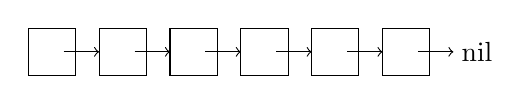
\begin{tikzpicture}[scale=3]
  \foreach \x in {-2, -1.7, ..., -0.4} {
    \draw (\x cm, 1cm) +(-0.1, -0.1) rectangle ++(0.1, 0.1);
    \draw[->] (\x cm, 1cm) +(0.05, 0) -- +(0.2, 0);
  }
  \draw (-0.2cm, 1cm) node {nil};
\end{tikzpicture}
\caption{Linked-list}
\label{fig:linked-list}
\end{figure}

Because every node links to the next one or nil, list is also called as `linked-list'. In the tradition of computer programs, linked-list is often defined through the record data structure\footnote{In most cases, the data stored in list have the same type. However, there is also heterogeneous list, like the list in Lisp for example.}, for example:

\begin{lstlisting}
Node of A:
    key: A
    next: Node of A
\end{lstlisting}

We can also understand the list as isomorphism of natural numbers. According to the first Peano axiom, nil is corresponding to zero; Based on the second Peano axiom, for any list, we can apply \texttt{cons}, to link a new element of type A to the left. We can treat \texttt{cons} corresponding to \texttt{succ} to the natural numbers. There are two different things. First, list is augmented with elements of type A. List \texttt{cons(1, cons(2, cons(3, nil)))} and \texttt{cons(2, cons(1, cons(3, nil)))}; List \texttt{cons(1, cons(4, cons(9, nil)))} and \texttt{cons('a', cons('b', cons('c', nil)))} are all different lists. Second, new element is not added to the right at tail, but is added to the left on head. Different from the intuition, the list grows to the left but not to the right.

It's not convenient to represent long list with nested \texttt{cons}. We simplify \texttt{cons(1, cons(2, cons(3, nil)))} to [1, 2, 3], and use symbol `:' for \texttt{cons}. This list can also be written as 1:[2, 3] or 1:(2:(3:nil)). When type A is character, we use string in quote to represent this special type of list. For example, ``hello'' is the simplified form for ['h', 'e', 'l', 'l', 'o'].

Similar to add defined for natural numbers, we can define the concatenation for lists as the following.

\be
\begin{array}{l}
nil \doubleplus y = y \\
cons(a, x) \doubleplus y = cons(a, x \doubleplus y)
\end{array}
\ee

There are two rules for list concatenation. First, empty list concatenates any list produces the same list; second, when concatenate the `successor' of a list to another one, it equals to firstly concatenate the two lists, then take the successor. Compare to the add for natural numbers, the definition of list concatenation is mirrored symmetric.

\begin{figure}[htbp]
\begin{tabular}{r|l}
$nil \doubleplus y = y$ & $a + 0 = a$ \\
$cons(a, x) \doubleplus y = cons(a, x \doubleplus y)$ & $a + succ(b) = succ(a + b)$
\end{tabular}
\caption{The list concatenation and natural number adding are mirrored symmetric.}
\end{figure}

With the hint of symmetry, we can prove the associative law for list concatenation through the induction axiom. To prove $(x \doubleplus y) \doubleplus z = x \doubleplus (y \doubleplus z)$, we first prove it holds for $x = nil$.

\[
\begin{array}{lll}
(nil \doubleplus y) \doubleplus z & = y \doubleplus z & \text{1st equation of $\doubleplus$} \\
 & = nil \doubleplus (y \doubleplus z) & \text{1st equation of $\doubleplus$ (backward)}
\end{array}
\]

For the induction case, assume $(x \doubleplus y) \doubleplus z = x \doubleplus (y \doubleplus z)$ holds. We want to prove that $((a:x) \doubleplus y) \doubleplus z = (a:x) \doubleplus (y \doubleplus z)$.

\[
\begin{array}{rll}
((a:x) \doubleplus y) \doubleplus z & = (a:(x \doubleplus y)) \doubleplus z & \text{2nd equation of $\doubleplus$} \\
 & = a:((x \doubleplus y) \doubleplus z) & \text{2nd equation of $\doubleplus$} \\
 & = a:(x \doubleplus (y \doubleplus z)) & \text{induction assumption} \\
 & = (a:x) \doubleplus (y \doubleplus z) & \text{2nd equation of $\doubleplus$ (backward)}
\end{array}
\]

With this, we proved the list concatenation is associative. Different from the natural numbers however, list concatenation is not commutative\footnote{This is the reason why we avoid using symbol + for concatenation. But many programming languages use the + sign. It causes potential issues in practice.}. For example $[2, 3 ,5] \doubleplus [7, 11] = [2, 3, 5, 7, 11]$, but when change the order, the result is $[7, 11] \doubleplus [2, 3, 5] = [7, 11, 2, 3, 5]$.

Consider the similarity to the natural numbers, we can also define the abstract folding operation for lists. Corresponding to the abstract start value $c$ and the abstract binary operation $h$, we define the recursive scheme as below.

\be
\begin{array}{l}
f(nil) = c \\
f(cons(a,x)) = h(a, f(x))
\end{array}
\ee

As the next step, let $f = foldr(c, h)$, then we can abstract the list folding. We name it as $foldr$ to call out the folding starts from right to left.

\be
\begin{array}{l}
foldr(c, h, nil) = c \\
foldr(c, h, cons(a,x)) = h(a, foldr(c, h, x))
\end{array}
\ee

We can define varies of list manipulations with $foldr$. The followings are to sum and multiply all the elements in list.

\be
\begin{array}{l}
sum = foldr(0, +) \\
product = foldr(1, \times)
\end{array}
\ee

We can understand how $sum$ behaves with examples. First is about empty list, $sum(nil) = foldr(0, +, nil) = 0$. Then the list with some elements:

\[
\begin{array}{rl}
sum([1, 3, 5, 7]) & = foldr(0, +, 1:[3, 5, 7]) \\
 & = 1 + foldr(0, +, 3:[5, 7]) \\
 & = 1 + (3 + foldr(0, +, 5:[7])) \\
 & = 1 + (3 + (5 + foldr(0, +, cons(7, nil)))) \\
 & = 1 + (3 + (5 + (7 + foldr(0, +, nil)))) \\
 & = 1 + (3 + (5 + (7 + 0))) \\
 & = 16
\end{array}
\]

We can measure the length of the list with $sum$. It essentially maps a list to a natural number.

\be
\begin{array}{l}
one(a) = 1 \\
length = sum \circ foldr(0, one)
\end{array}
\ee

Where function $one$ is called as {\em constant} function. It always returns 1 for whatever variables. We can use $|x| = length(x)$ to represent the length of a given list. The next example shows we can use $foldr$ to define list concatenation.

\be
(\doubleplus y) = foldr(y, cons)
\ee

It is corresponding to the $(+m)$ operation for natural number. Further, similar to the multiplication of natural numbers, we can define the `multiplication' for lists, concatenate all sub-lists in a list.

\be
concat = foldr(nil, \doubleplus)
\ee

When apply $concat([[1, 1], [2, 3, 5], [8]])$, the result is $[1, 1, 2, 3, 5, 8]$. At the end of this section, we'll define two important list operations with $foldr$, filtering and mapping\footnote{Different from one to one mapping, the map defined here is one direction only. For example, the map from a string to its length is one direction. The reverse map does not exist.}. Filter is to compose a new list from the elements that satisfy a given predication. In order to realize filtering, we need introduce the conditional expression\footnote{Also known as McCarthy conditional form, or McCarthy formalism. It was introduced by the computer scientist, the inventor of Lisp, John McCarthy in 1960.}. It's written as $(p \mapsto f, g)$. When give variable $x$, if the predication $p(x)$ holds, then the result is $f(x)$, else it's $g(x)$. We also use if $p(x)$ then $f(x)$ else $g(x)$ for conditional expression.

\be
filter(p) = foldr(nil, (p \circ 1st \mapsto cons, 2nd))
\ee

Let's use an example to understand how this definition works. We want to select all even numbers from a list $filter(even, [1, 4, 9, 16, 25])$. Like expansion process in $sum$, the filtering expands to $h(1, h(4, h(9, ...)))$ till the right end $cons(25, nil)$. According to the definition of $foldr$, the result is $c$ when the list is $nil$. So the next step is to compute $h(25, nil)$, where $h$ is the conditional expression. When apply $even \circ 1st$ to the pair $(25, nil)$, function $1st$ picks 25, as it's odd, the predication $even$ does not hold. Based on the conditional expression, $2nd$ is evaluated and gives the result $nil$. Then we enter the upper level to compute $h(16, nil)$. Function $1st$ extracts the number 16, as 16 is even, the predicate $even$ holds, so the conditional expression sends to $cons(16, nil)$, which produces the list $[16]$. Then we enter one more upper level to compute $h(9, [16])$, the conditional expression sends to $2nd$, which again produces $[16]$. The computation enters to $h(4, [16])$ next. The conditional expression sends to $cons(4, [16])$, which produces the list $[4, 16]$. The computation finally reach to the top level $h(1, [4, 16])$. The conditional expression sends to $2nd$, which produces the final result $[4, 16]$.

The concept of mapping is to transform every element in one list to another value through a function $f$, and form a new list. That is $map(f, \{x_1, x_2, ..., x_n\})$ = $\{f(x_1)$, $f(x_2)$, ..., $f(x_n)\}$. It can be defined with $foldr$ as below.

\be
\begin{array}{l}
map(f) = foldr(nil, h) \\
h(x, c) = cons(f(x), c)
\end{array}
\ee

We call the operation that applies a function to the first value in a pair as `$first$', that is $first(f, (x, y)) = (f(x), y)$. We'll come back to it in the chapter of category theory. With $first$, map can be defined as $map(f) = foldr(nil, cons \circ first(f))$.

\begin{Exercise}\label{ex:foldr}
\Question{What does the expression $foldr(nil, cons)$ define?}
\Question{Read in a sequence of digits (string of digit numbers), convert it to decimal with $foldr$. How to handle hexadecimal digit and number? How to handle the decimal point?}
\Question{Jon Bentley gives the maximum sum of sub-vector puzzle in {\em Programming Pearls}. For integer list $\{x_1, x_2, ..., x_n\}$, find the range $i, j$, that maximizes the sum of $x_i + x_{i+1} + ... + x_j$. Solve it with $foldr$.}
\Question{The longest sub-string without repeated characters. Given a string, find the longest sub-string without any repeated characters in it. For example, the answer for string ``abcabcbb'' is ``abc''. Solve it with $foldr$.}
\end{Exercise}

\begin{Answer}[ref={ex:foldr}]
\Question{What does the expression $foldr(nil, cons)$ define?

It defines the list itself.
}
\Question{Read in a sequence of digits (string of digit numbers), convert it to decimal with $foldr$. How to handle hexadecimal digit and number? How to handle the decimal point?

If the lowest digit is on the left, and the highest digit on the right in the input list, we can convert it as below:

\[
foldr\ (c\ d \mapsto 10d + c)\ 0
\]

However, if the lowest digit is on the right, and the elements in the list are characters but not digit, then we need adjust it to:

\[
1st \circ foldr\ (c, (d, e) \mapsto ((toInt\ c)e + d, 10e))\ (0, 1)
\]

We can make it process the hexadecimal numbers by replacing 10 to 16 in this definition. When meet the decimal point, we can divide $d$, the result so far, by $e$ to calculate the fractional part value.

\[
1st \circ foldr\ h\ (0, 1)
\]

where

\[
h\ (c, (d, e)) = \begin{cases}
c = '.' & (d / e, 1) \\
\text{otherwise} & ((toFloat\ c)e + d, 10e) \\
\end{cases}
\]
}
\Question{Jon Bentley gives the maximum sum of sub-vector puzzle in {\em Programming Pearls}. For integer list $\{x_1, x_2, ..., x_n\}$, find the range $i, j$, that maximizes the sum of $x_i + x_{i+1} + ... + x_j$. Solve it with $foldr$.

If all numbers are positive, then the maximum sum is the sum of the whole list. This is because addition is monotone increasing upon positive numbers. If all numbers are negative, then the maximum sum should be zero, which is the sum of empty list. For any sub-list, the sum increases when add a positive number, while it decreases when add a negative number. We can maintain two things during folding: one is the maximum sum found so far $S_m$, the other is the sum of the sub-list till the current number being examined $S$. By adding the next element, if $S$ exceeds $S_m$, it means we found a larger sub-list sum. Hence we replace $S_m$ with $S$; If $S$ becomes negative, it means we complete the previous sub-list, and should start a new one.

\blre
max_s & = & 1st \circ foldr\ f\ (0, 0) \\
\text{where}: & & f\ x\ (S_m, S) = (S_m' = \max(S_m, S'), S' = \max(0, x + S)) \\
\elre

Here is the example program implements this solution.

\lstset{frame=single}
\begin{lstlisting}
maxSum :: (Ord a, Num a) => [a] -> a
maxSum = fst . foldr f (0, 0) where
  f x (m, mSofar) = (m', mSofar') where
    mSofar' = max 0 (mSofar + x)
    m' = max mSofar' m
\end{lstlisting}

If want to return the sub-list together with the maximum sum, we can maintain two pairs $P_m$ and $P$ during folding, each pair contains the sum and the sub-list $(S, L)$.

\blre
max_s & = & 1st \circ foldr\ f\ ((0, [\ ]), (0, [\ ])) \\
\text{where}: & & f\ x\ (P_m, (S, L)) = (P_m' = \max(P_m, P'), P' = \max((0, [\ ]), (x + S, x \cons L))) \\
\elre
}
\Question{The longest sub-string without repeated characters. Given a string, find the longest sub-string without any repeated characters in it. For example, the answer for string ``abcabcbb'' is ``abc''. Solve it with $foldr$.

We give two methods. One solution is to maintain the longest sub-string without repeated characters during folding, record and check if the character $c$ has met before and its last appeared position. If $c$ never occurred, or it appears before the current sub-string we are examining, then we append it to the current sub-string, and compare with the longest one we've found so far. Otherwise, it means the current sub-string contains a repeated character, we need go back to its last occurred position, move ahead one, then restart searching.

\[
longest(S) = fst2 \circ foldr\ f\ (0, |S|, |S|, \varnothing)\ zip(\{1, 2, ...\}, S)
\]

Where folding starts from a tuple of 4 elements. It contains the length of the longest sub-string we found so far, the right boundary of the longest sub-string, the right boundary of the current sub-string, and a map recorded the last occurred position for different characters. Function $fst2$ extract the first two elements from the tuple as result. To obtain the position of each character easily during folding, we $zip$ the string $S$ and natural number sequence together. The most critical function $f$ is defined as below:

\[
f\ (i, c)\ (n_{max}, e_{max}, e, Idx) = (n_{max}', e_{max}', e', Idx[c] = i)
\]

where:

\[ \begin{array}{l}
n_{max}' = max(n_{max}, e' - i + 1) \\
e' = \begin{cases}
  c \notin Idx: & e \\
  Idx[c] = j: & min(e, j - 1) \\
  \end{cases} \\
e_{max}' = \begin{cases}
  e' - i + 1 > n_{max}: & e' \\
  \text{otherwise}: & e_{max} \\
  \end{cases} \\
\end{array} \]

Here is an example program implement this solution. It returns the maximum length and the end position of the sub-string.

\lstset{frame=single}
\begin{lstlisting}
longest :: String -> (Int, Int)
longest xs = fst2 $ foldr f (0, n, n, Map.empty::(Map Char Int))
                      (zip [1..] xs) where
  fst2 (len, end, _, _) = (len, end)
  n = length xs
  f (i, x) (maxlen, maxend, end, pos) =
      (maxlen', maxend', end', Map.insert x i pos) where
    maxlen' = max maxlen (end' - i + 1)
    end' = case Map.lookup x pos of
      Nothing -> end
      Just j -> min end (j - 1)
    maxend' = if end' - i + 1 > maxlen then end' else maxend
\end{lstlisting}

We record ending position because $foldr$ starts from right. While the traditional way starts from the left, for example:

\begin{algorithmic}
\Function{Longest}{$S$}
  \State $Idx \gets \varnothing$
  \State $n_{max} \gets 0, s_{max} \gets 0, s \gets 0$
  \For{$i \in \{0, 1, ... |S|\}$}
    \If{$S[i] \in Idx$}
      \State $j \gets Idx[S[i]]$
      \State $s = max(s, j + 1)$
    \EndIf
    \If{$i - s + 1 > n_{max}$}
      \State $s_{max} \gets s$
    \EndIf
    \State $n_{max} \gets max(n_{max}, i - s + 1)$
    \State $Idx[S[i]] = i$
  \EndFor
  \State \Return $S[s_{max} ... s_{max} + n_{max}]$
\EndFunction
\end{algorithmic}

The second method is a number theory solution by leveraging prime numbers. We map each unique character $c$ to a prime number $p_c$. For any string $S$, we can calculate the product of prime numbers mapped from its characters:

\[
P = \displaystyle \prod_{c \in S} p_c
\]

Therefore, for any new character $c'$, we can check whether the corresponding prime number $p'$ divides $P$ or not to know if $c'$ appears in $S$. Based on this fact, we can design an algorithm. It maintains the product of primes during folding. When there is a character, that its corresponding prime number divides the product, we then find a repeated character. We need drop off the part containing the repeated character and go on folding. During this process, we also need update the longest sub-string.

\[
longest = fst \circ foldr\ f\ ((0, [\ ]), (0, [\ ]), 1)
\]

Where the folding starts from a tuple of three elements. The first two are pairs, represent the longest sub-string (length and content), and the current sub-string. The last one in the tuple is the product of primes, starts from 1. Function $f$ is defined as the following:

\[
f\ c\ (m, (n, C), P) = \begin{cases}
  p_c | P : & update(m, (n + 1, c : C), p_c \times P) \\
  \text{otherwise}: & update(m, (|C'|, C'), \displaystyle \prod_{x \in C'} p_x) \\
\end{cases}
\]

where:

\[ \begin{array}{l}
update(a, b, P) = (max(a, b), b, P) \\
C' = c : takeWhile\ (\neq c)\ C \\
\end{array} \]
}
\end{Answer}

\section{Form and structure}

%\begin{wrapfigure}{R}{0.3\textwidth}
\begin{figure}[htbp]
 \centering
 \includegraphics[scale=1.0]{img/the-school-of-athens}
 \caption{Raphael, School of Athens (part)}
 \label{fig:the-school-of-athens}
\end{figure}
%\end{wrapfigure}

We illustrated several conclusions with geometry figures in this chapter, like the associative law, the commutative law, and the Fibonacci spiral. We want to express the beauty of isomorphism. Aristotle said
``The chief forms of beauty are order and symmetry and definiteness, which the mathematical sciences demonstrate in a special degree.'' ({\em Metaphysic}) Like geometry, with Peano's work, natural numbers can also be built on top of the axioms. We use the similarity of natural numbers and lists to demonstrate the beauty of symmetry. When the Italian Renaissance artist Raphael created the world famous fresco {\em School of Athens}, he used the same approach of isomorphism by inventing a system of iconography. Many ancient Greece philosophers were illustrated with the figures in Raphael's time of Renaissance. The center figures are Plato and his student Aristotle. Of which Plato is depicted in the image of Leonardo da Vinci; Aristotle is in the image of Giuliano da Sangallo. They were all great artists in Renaissance. The elder Plato is walking alongside Aristotle with his right hand figure point up, while Aristotle is stretching his hand forward. It is popularly thought that their gestures indicate central aspects of their philosophies, for Plato, his Theory of Forms, and for Aristotle, his empiricist views, with an emphasis on concrete particulars. Plato argues a sense of timelessness while Aristotle looks into the physicality of life and the present realm. Below the steps in the middle, the great philosopher Heraclitus leans the box and meditates. He is famous for the thoughts about simple dialectics and materialism. The image of Heraclitus is another great artist Michelangelo in Renaissance. The front left is centered on the great mathematician Pythagoras. He is writing something. On the right side of Pythagoras is a blond young man in a white cloak, considered to be Francisco Maria della Rovere. He was Ulbino's future Grand Duke. The center of the bottom right is the great mathematician Euclid with a compass in hand (or Archimedes in other opinion), he is surrounded by Ptolemy, the great astronomer with the celestial sphere in hand. The opposite is the painter Raphael's fellow villager, the architect Bramante. The one who wore a white hat on the right is the painter Sodom, the young man next to him with half head and a hat on his head, is the painter, Raphael himself. This reminds us the great musician Bach, who wrote his name B-A-C-H in his work `The Art of Fugue' (Die Kunst der Fuge in German). School of Athens reflects the ancient Greece art and philosophy with the figures in the time of Renaissance. It is the multiple levels of isomorphism of form and content, structure and thoughts. It is seen as ``Raphael's masterpiece and the perfect embodiment of the classical spirit of the Renaissance''.

\begin{Exercise}\label{ex:fibonacci-matrix}
\Question{In the fold definition of Fibonacci numbers, the successor is computed as $(m', n') = (n, m + n)$. It is essentially matrix multiplication:
\[
\begin{pmatrix} m' \\ n' \end{pmatrix} =
\begin{pmatrix} 0 & 1 \\ 1 & 1 \end{pmatrix}
\begin{pmatrix} m \\ n \end{pmatrix}
\]
Where it starts from $(0, 1)^T$. Then the Fibonacci numbers is isomorphic to natural numbers under the matrix multiplication:
\[
\begin{pmatrix}F_n \\ F_{n+1} \end{pmatrix} = \begin{pmatrix} 0 & 1 \\ 1 & 1 \end{pmatrix}^n\begin{pmatrix} 0 \\ 1 \end{pmatrix}
\]
Write a program to compute the power of 2-order square matrix, and use it to give the $n$-th Fibonacci number.}
\end{Exercise}

\begin{Answer}[ref = {ex:fibonacci-matrix}]
\Question{In the fold definition of Fibonacci numbers, the successor is computed as $(m', n') = (n, m + n)$. It is essentially matrix multiplication:
\[
\begin{pmatrix} m' \\ n' \end{pmatrix} =
\begin{pmatrix} 0 & 1 \\ 1 & 1 \end{pmatrix}
\begin{pmatrix} m \\ n \end{pmatrix}
\]
Where it starts from $(0, 1)^T$. Then the Fibonacci numbers is isomorphic to natural numbers under the matrix multiplication:
\[
\begin{pmatrix}F_n \\ F_{n+1} \end{pmatrix} = \begin{pmatrix} 0 & 1 \\ 1 & 1 \end{pmatrix}^n\begin{pmatrix} 0 \\ 1 \end{pmatrix}
\]
Write a program to compute the power of 2-order square matrix, and use it to give the $n$-th Fibonacci number.

First we need define multiplication for square matrix of order 2, and the multiplication between square matrix and vector:

\[
\begin{pmatrix}
a_{11} & a_{12} \\
a_{21} & a_{22} \\
\end{pmatrix}
\times
\begin{pmatrix}
b_{11} & b_{12} \\
b_{21} & b_{22} \\
\end{pmatrix}
=
\begin{pmatrix}
a_{11} b_{11} + a_{12} b_{21} & a_{11} b_{12} + a_{12} b_{22} \\
a_{21} b_{11} + a_{22} b_{21} & a_{21} b_{12} + a_{22} b_{22} \\
\end{pmatrix}
\]

and

\[
\begin{pmatrix}
a_{11} & a_{12} \\
a_{21} & a_{22} \\
\end{pmatrix}
\times
\begin{pmatrix}
b_{1} \\
b_{2} \\
\end{pmatrix}
=
\begin{pmatrix}
a_{11} b_{1} + a_{12} b_{2} \\
a_{21} b_{1} + a_{22} b_{2} \\
\end{pmatrix}
\]

When calculate the $n$-th power of $M^n$, we need not repeat multiplication $n$ times. If $n = 4$, we can first calculate $M^2$, then multiply the result to itself to obtain $(M^2)^2$. There are total two times of multiplication; If $n = 5$, we only need compute $M^4 \times M$, hence there are three times of multiplication. We can recursively compute the exponential fast based on $n$'s parity.

\[
M^n = pow(M, n, I)
\]

Where $I$ is the identical square matrix of order 2: $\displaystyle \begin{pmatrix} 1 & 0 \\ 0 & 1\end{pmatrix}$, and the function $pow$ is defined as below:

\[
pow(M, n, A) = \begin{cases}
n = 0: & A \\
n\ \text{is even}: & pow(M \times M, \dfrac{n}{2}, A) \\
\text{otherwise}: & power(M \times M, \lfloor \dfrac{n}{2} \rfloor, M \times A)\\
\end{cases}
\]

In fact, we can represent $n$ in binary format, then perform folding on these 0, 1 bits to compute $M^n$ fast.
}
\end{Answer}

\ifx\wholebook\relax \else
\section{Answer}
\shipoutAnswer

\begin{thebibliography}{99}

\bibitem{wiki-number}
Wikipedia. ``History of ancient numeral systems''. \url{https://en.wikipedia.org/wiki/History_of_ancient_numeral_systems}

\bibitem{Calvin-Clawson-1994}
Calvin C Clawson. ``The Mathematical Traveler, Exploring the Grand History of Numbers''. Springer. 1994, ISBN: 9780306446450

\bibitem{wiki-babylonian-num}
Wikipedia. ``Babylonian numerals''. \url{https://en.wikipedia.org/wiki/Babylonian_numerals}

\bibitem{M-Kline-2007}
Morris Kline ``Mathematics: The Loss of Certainty''. Oxford University Press, 1980. 0-19-502754-X.

\bibitem{GEB}
Douglas R. Hofstadter ``Gödel, Escher, Bach: An Eternal Golden Braid''. Basic Books; Anniversary edition (February 5, 1999). ISBN: 978-0465026562

\bibitem{Bird97}
Richard Bird, Oege de Moor. ``Algebra of Programming''. University of Oxford, Prentice Hall Europe. 1997. ISBN: 0-13-507245-X.

\bibitem{Gusen2014}
顾森\ 《浴缸里的惊叹》People's postal Press. 2014, ISBN: 9787115355744

\end{thebibliography}

\expandafter\enddocument
%\end{document}

\fi
